\section{1174079 -Chandra Kirana Poetra}
\subsection{Teori}
\begin{enumerate}

	\item Jelaskan apa itu klasifikasi teks, sertakan gambar ilustrasi buatan sendiri.
	\hfill\break
	Klasifikasi teks merupakan suatu proses dalam memberikan tag atau kategori pada suatu teks berdasarkan konten. klasifikasi teks merupakan salah satu bagian dari natural language processing yang mencakup analisis, labeling, deteksi spam dan intent detection. Untuk ilustrasinya bisa dilihat pada gambar berikut : 

	\begin{figure}[H]
	\centering
		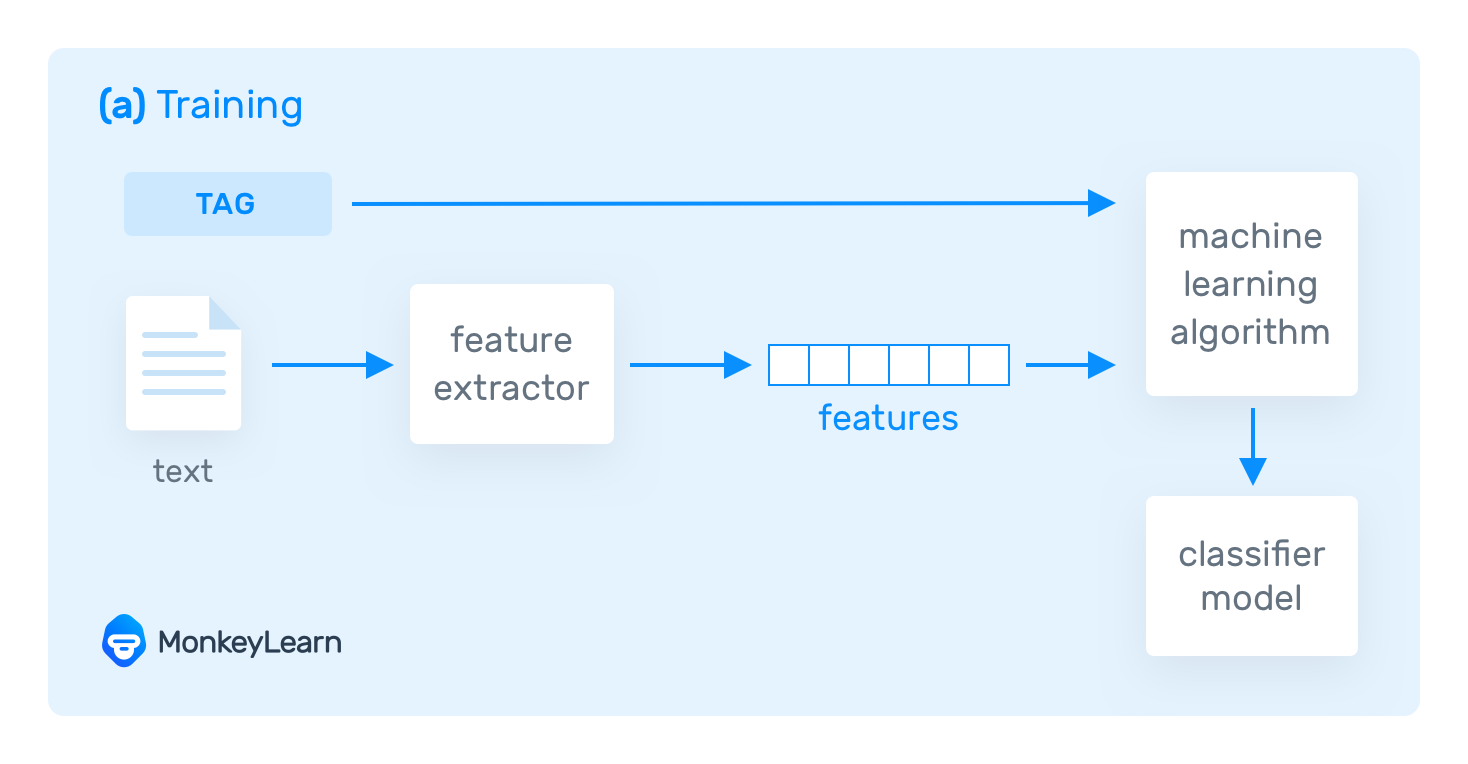
\includegraphics[width=4cm]{figures/1174079/4/klasifikasiteks1.png}
		\caption{Klasifikasi teks.}
	\end{figure}
	\begin{figure}[H]
	\centering
		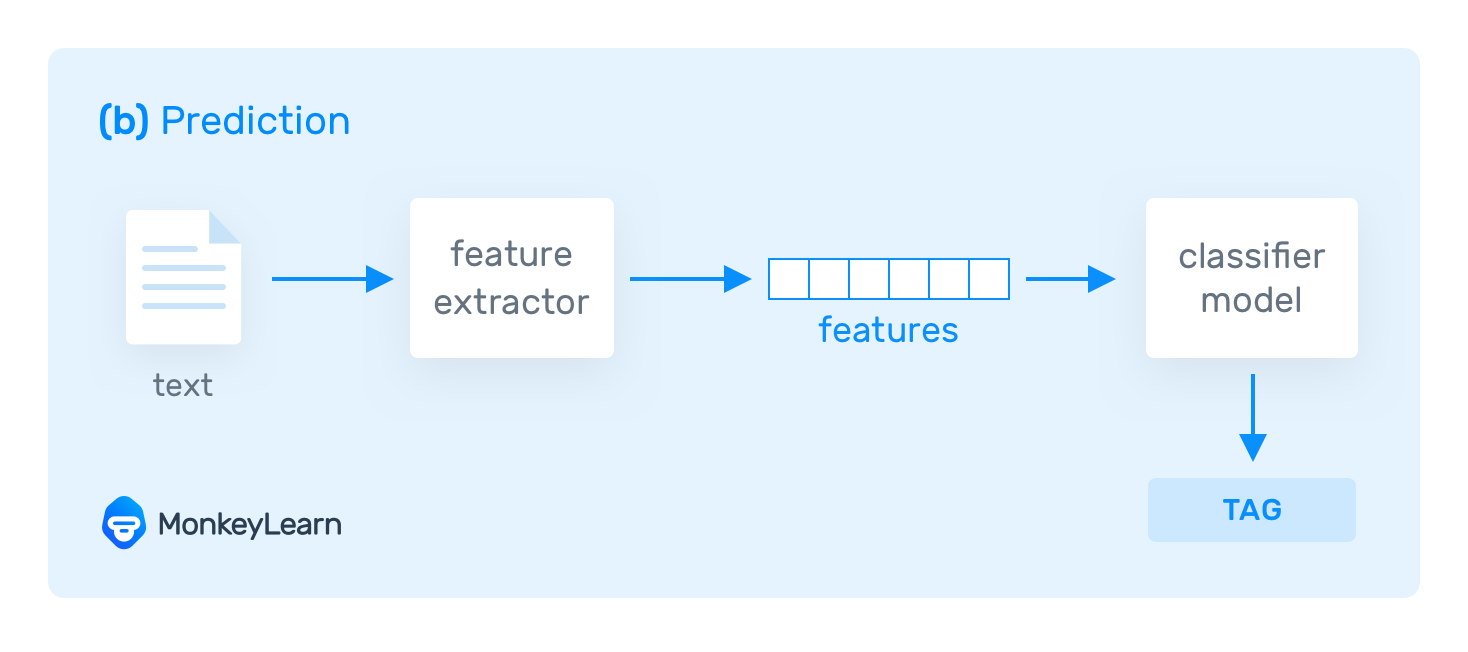
\includegraphics[width=4cm]{figures/1174079/4/klasifikasiteks2.png}
		\caption{Klasifikasi teks.}
	\end{figure}

	\item Jelaskan mengapa hal ini bisa terjadi, klasifikasi bunga tidak bisa digunakan untuk machine learning, sertakan ilustrasi gambar sendiri.
	\hfill\break
	Karena meskipun bunga yang kita coba untuk klasifikasikan memiliki spesies yang sama, kebanyakan bunga sendiri memiliki bentuk ukuran yang berbeda beda sehingga akan membuat machine learning sulit diterapkan karena ukuran tidak bisa dijadikan sebagai salah satu parameter dalam machine learning.
\begin{figure}[H]
	\centering
		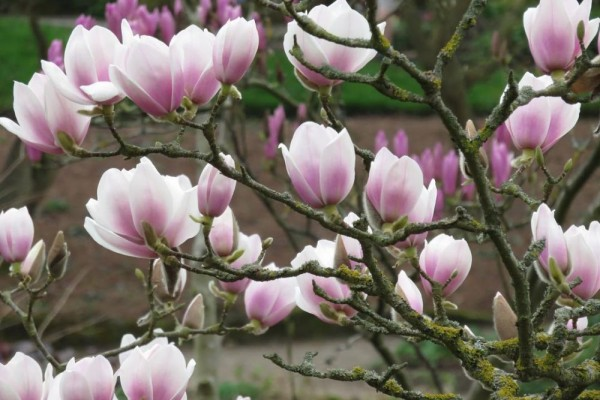
\includegraphics[width=4cm]{figures/1174079/4/bentukbunga.jpg}
		\caption{Ukuran Bunga yang berbeda-beda.}
	\end{figure}
	
	\item Jelaskan bagaimana yang dimaksud dengan teknik pembelajaran mesin pada teks yang digunakan dan sertakan ilustrasi buatan sendiri.
	\hfill\break
	Youtube menggunakan istilah yang disebut sebagai keyword yang nantinya kita isi didalam form pencarian yang ada kemudian akan muncul video yang terkait
	\begin{figure}[H]
	\centering
		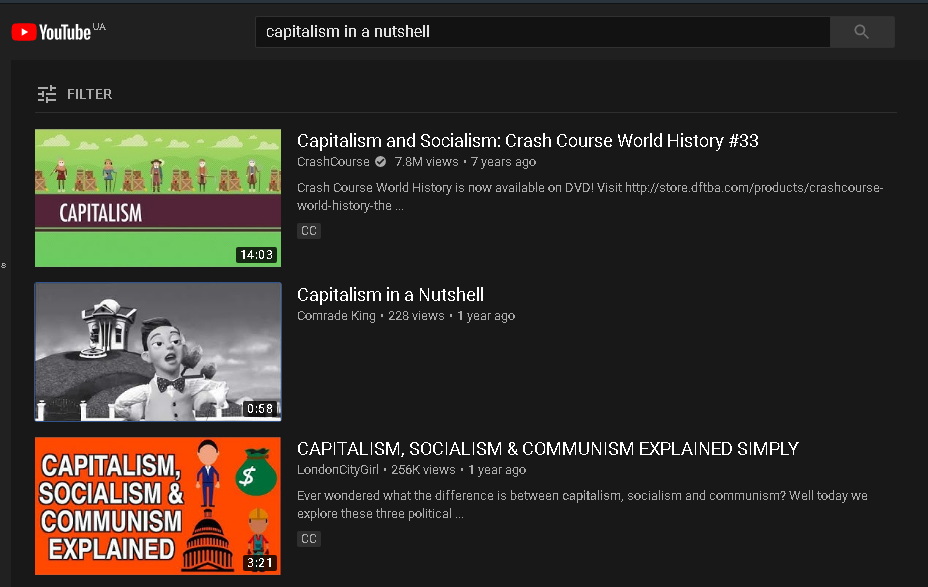
\includegraphics[width=4cm]{figures/1174079/4/klasifikasiteks3.PNG}
		\caption{Klasifikasi teks Youtube.}
	\end{figure}

	\item Jelaskan apa yang dimaksud vektorisasi data.
	\hfill\break
	vektorisasi merupakan suatu proses untuk mengkonversi suatu algoritma yang beroperasi pada satu value dalam satu waktu menjadi kebeberapa value dalam satu waktu

	\item Jelaskan apa yang dimaksud dengan bag of words dengan ilustrasi sendiri.
	\hfill\break
	Merupakan model untuk menyederhanakan data dalam bidang natural language processing dan juga pengambilan informasi. di model ini text direpresentasikan sebagai suatu kantong kata, mengabaikan grammer dan susunan kata tapi menyimpan value pengulangan apabila ada kata yang diulang. model ini digunakan pada bidang komputer

	\begin{figure}[H]
	\centering
		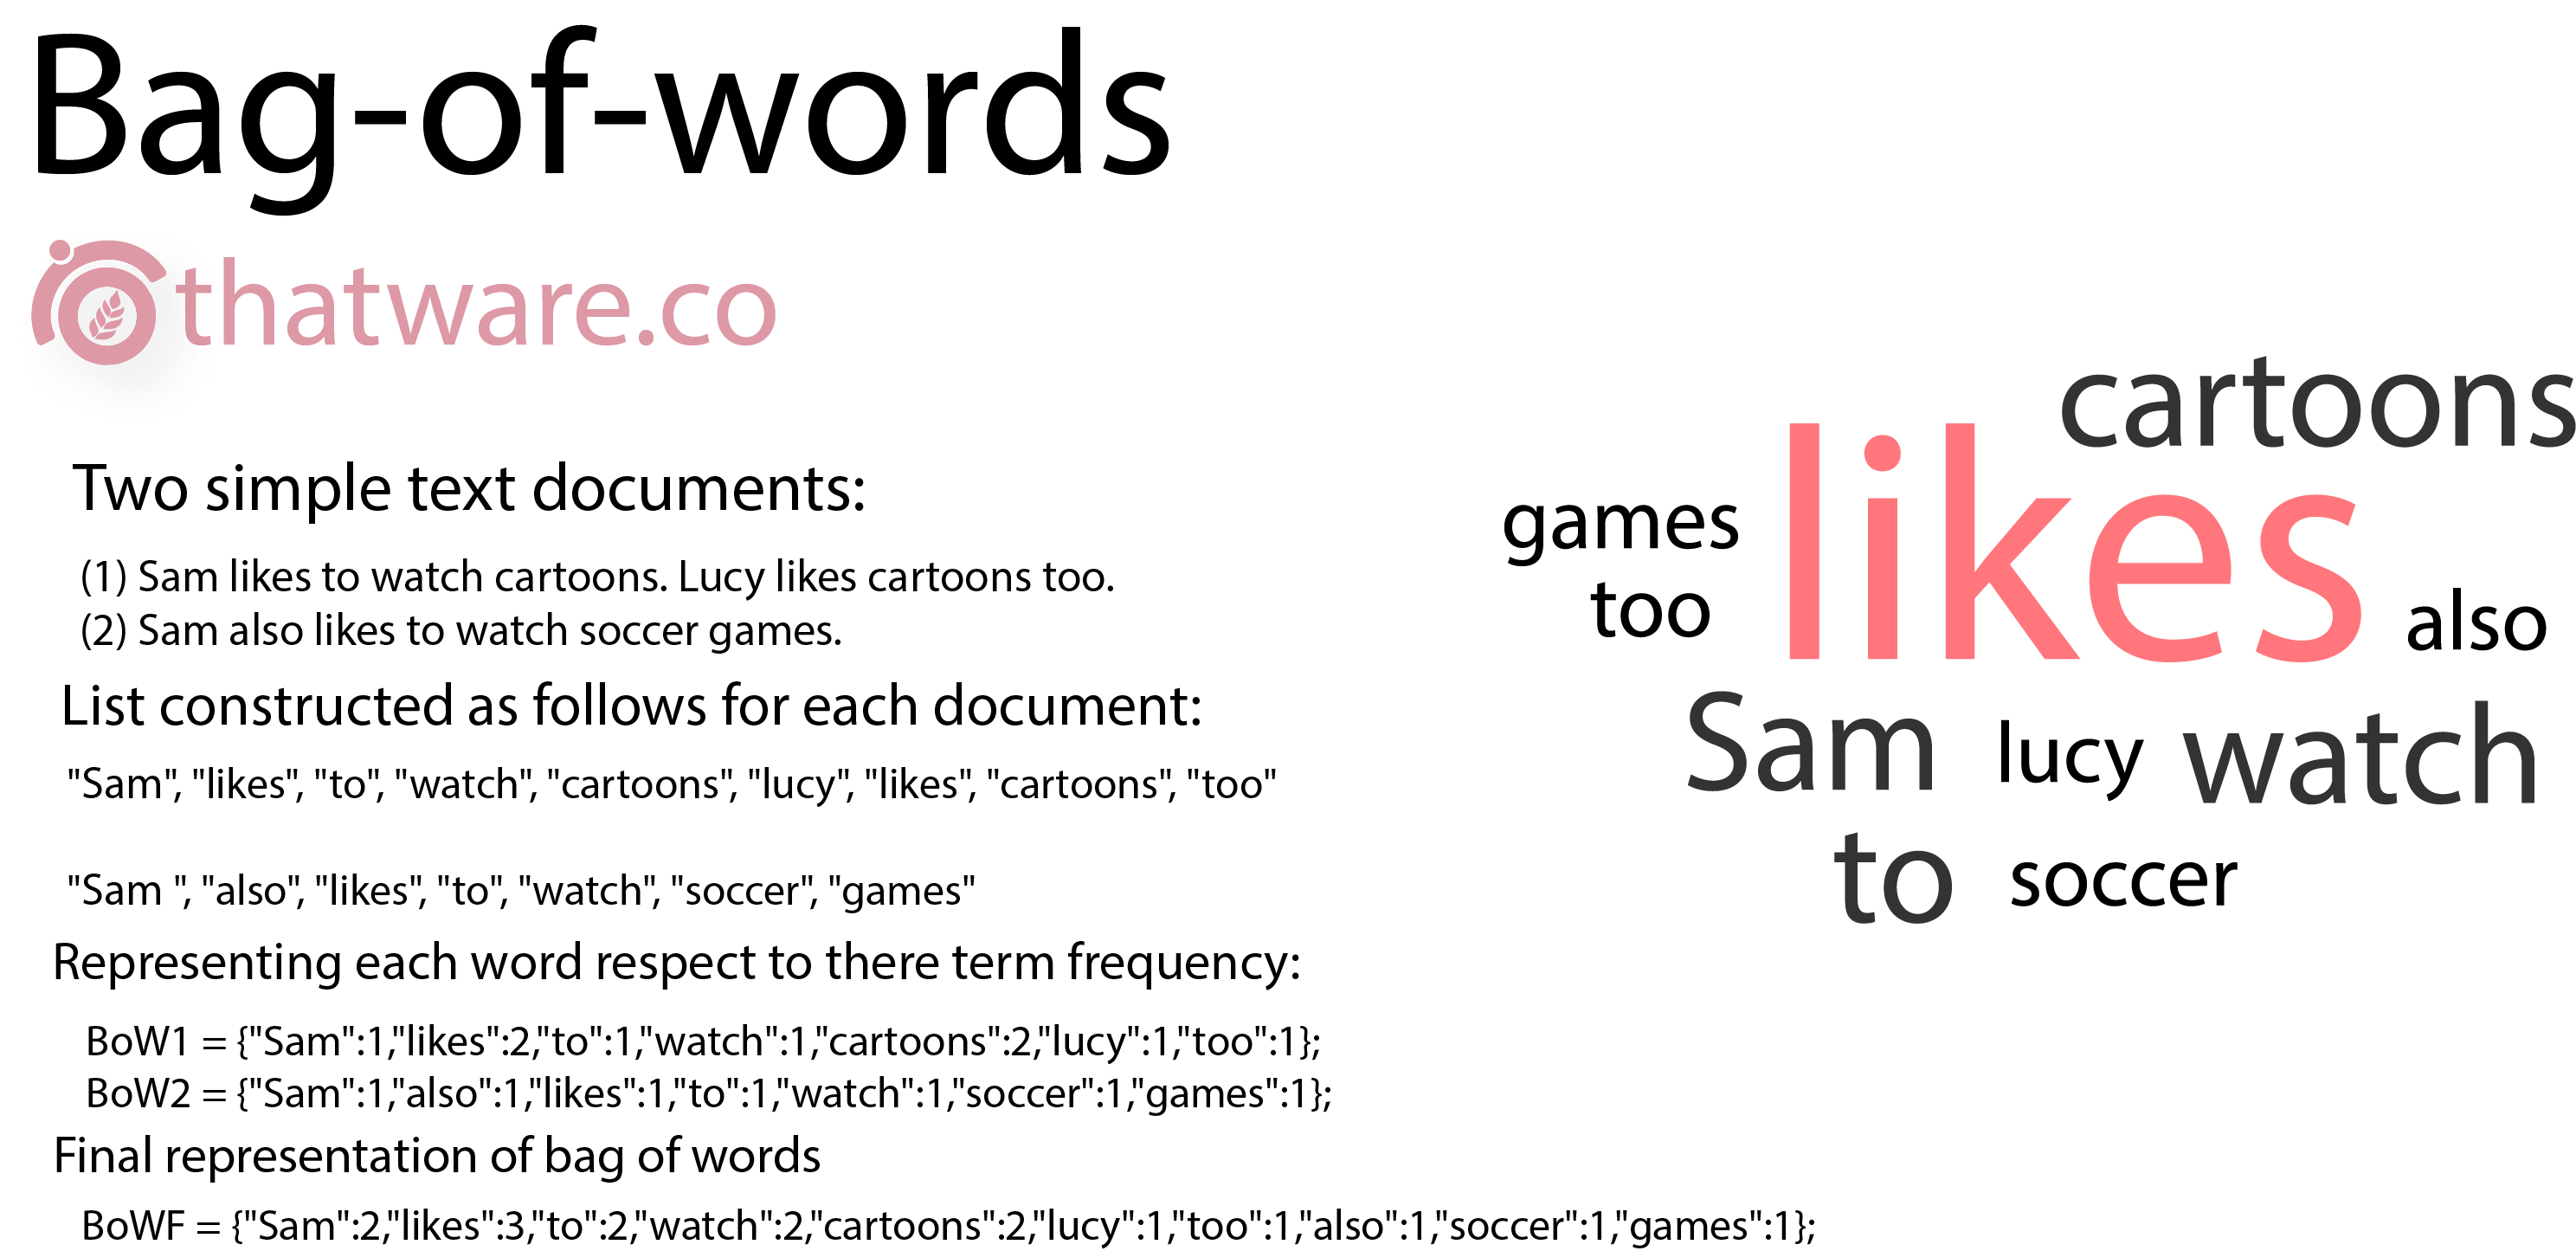
\includegraphics[width=4cm]{figures/1174079/4/bagofword.png}
		\caption{Bag of words.}
	\end{figure}

	\item Jelaskan apa yang dimaksud dengan TF-IDF.
	\hfill\break
	TF-IDF merupakan singkatan dari term frequency inverse document frequency yang merupakan statistik angka yang memiliki tujuan untuk memperlihatkan seberapa pentingnya suatu kata dalam suatu dokumen.

	\begin{figure}[H]
	\centering
		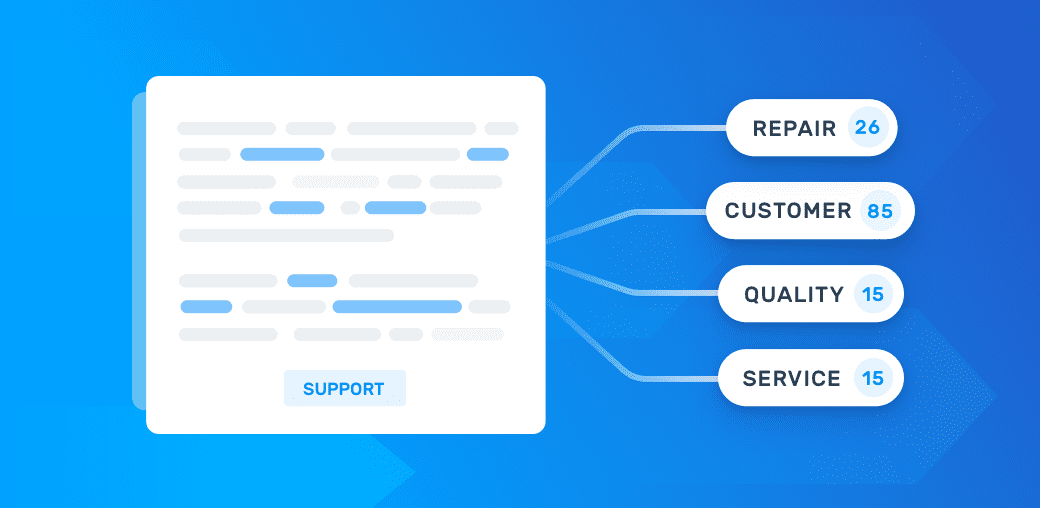
\includegraphics[width=4cm]{figures/1174079/4/TFIDF.png}
		\caption{TF-IDF.}
	\end{figure}
\end{enumerate}


\subsection{Praktek Program}
\subsubsection{Nomor 1}
\hfill\break
\lstinputlisting[firstline=8, lastline=10]{src/1174079/4/4.py}
\begin{figure}[H]
\centering
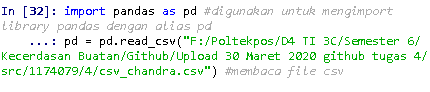
\includegraphics[width=4cm]{figures/1174079/4/soal1.PNG}
\caption{Nomor 1}
\end{figure}

\subsubsection{Nomor 2}
\hfill\break
\lstinputlisting[firstline=12, lastline=14]{src/1174079/4/4.py}
\begin{figure}[H]
\centering

\includegraphics[width=4cm]{figures/1174079/4/soal2.PNG}
\caption{Nomor 2}
\end{figure}

\subsubsection{Nomor 3}
\hfill\break
\lstinputlisting[firstline=16, lastline=40]{src/1174079/4/4.py}
\begin{figure}[H]
\centering
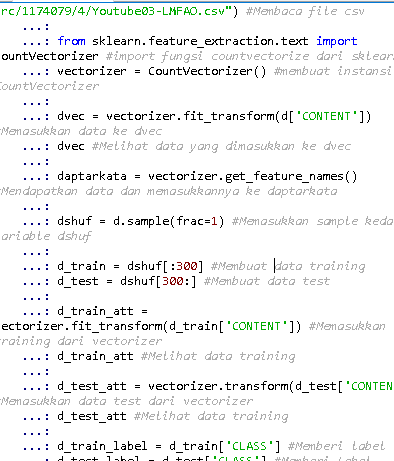
\includegraphics[width=4cm]{figures/1174079/4/soal3.PNG}
\caption{Nomor 3}
\end{figure}

\subsubsection{Nomor 4}
\hfill\break
\lstinputlisting[firstline=43, lastline=47]{src/1174079/4/4.py}
\begin{figure}[H]
\centering
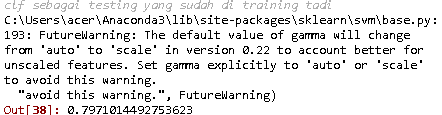
\includegraphics[width=4cm]{figures/1174079/4/soal4.PNG}
\caption{Nomor 4}
\end{figure}

\subsubsection{Nomor 5}
\hfill\break
\lstinputlisting[firstline=51, lastline=55]{src/1174079/4/4.py}
\begin{figure}[H]
\centering
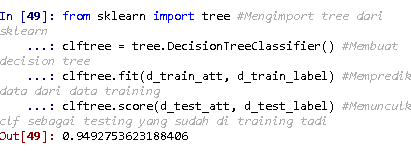
\includegraphics[width=4cm]{figures/1174079/4/soal5.PNG}
\caption{Nomor 5}
\end{figure}

\subsubsection{Nomor 6}
\hfill\break
\lstinputlisting[firstline=65, lastline=115]{src/1174079/4/4.py}
\begin{figure}[H]
\centering
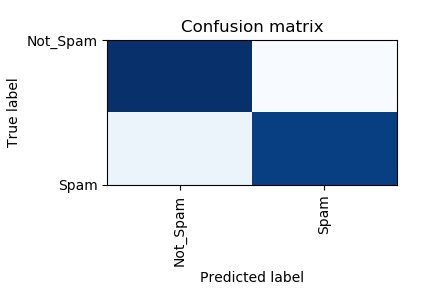
\includegraphics[width=4cm]{figures/1174079/4/soal6.PNG}
\caption{Nomor 6}
\end{figure}

\subsubsection{Nomor 7}
\hfill\break
\lstinputlisting[firstline=169, lastline=179]{src/1174079/4/4.py}
\begin{figure}[H]
\centering
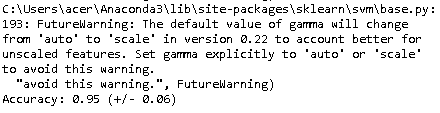
\includegraphics[width=4cm]{figures/1174079/4/soal7.PNG}
\caption{Nomor 7}
\end{figure}

\subsubsection{Nomor 8}
\hfill\break
\lstinputlisting[firstline=182, lastline=196]{src/1174079/4/4.py}
\begin{figure}[H]
\centering
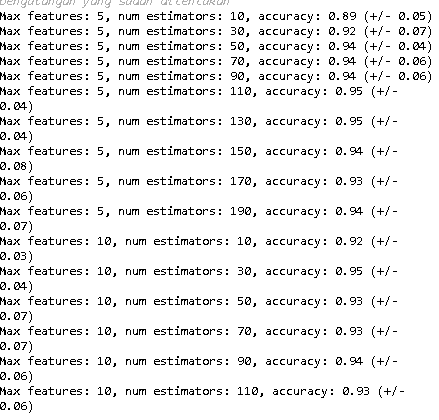
\includegraphics[width=4cm]{figures/1174079/4/soal8.PNG}
\caption{Nomor 8}
\end{figure}

\subsection{Penanganan Error}
\begin{enumerate}
	\item ScreenShoot Error
	\begin{figure}[H]
		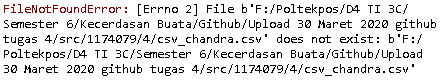
\includegraphics[width=4cm]{figures/1174079/4/error.PNG}
		\centering
		\caption{SyntaxError}
	\end{figure}
	\item Cara Penangan Error
	\begin{itemize}
		\item SyntaxError
		\hfill\break
		Memperbaiki typo dan mengecek nama file serta direktorinya
	\end{itemize}
\end{enumerate}

\subsection{Bukti Tidak Plagiat}
\begin{figure}[H]
\centering
	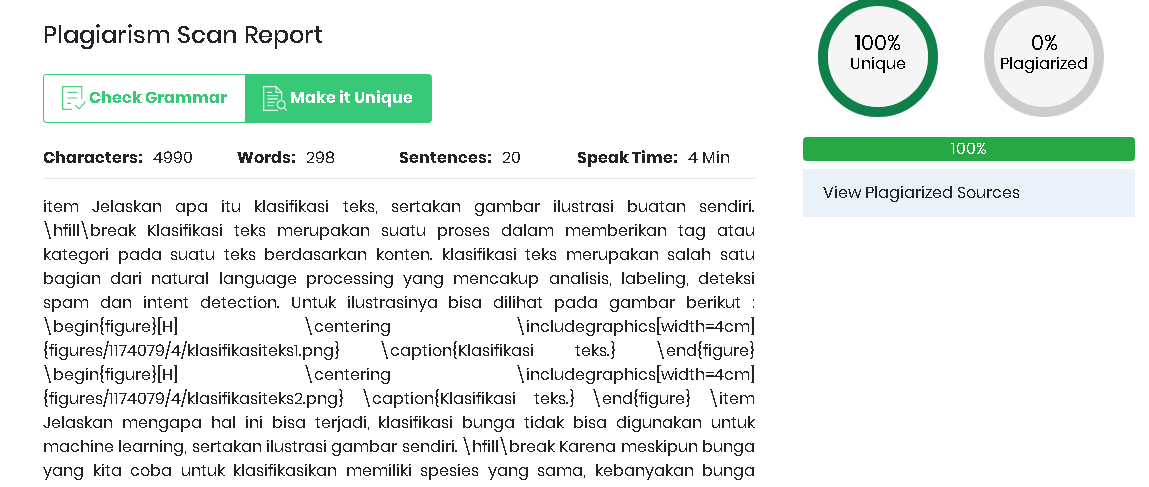
\includegraphics[width=4cm]{figures/1174079/4/plagiarisme.PNG}
	\caption{Bukti Tidak Melakukan Plagiat Chapter 4}
\end{figure}

\subsection{Link Youtube}
https://youtu.be/8vkMpgUVTQs

